Ante la imposibilidad de realizar la carga inalámbrica se tuvo una reunión con el cliente para discutir el proceder. El cliente indicó que el dato principal que se requiere del vuelo del ave es la posición.
Para la obtención de datos de la trayectoria del ave se propuso el siguiente esquema:
\Subsubsubsection{Módulos del Sistema de Seguimiento}
La propuesta se basa en cuatro partes, la mochila del ave,
 las bases de seguimiento, una base principal de seguimiento y la comunicación de esta con la base del nido.
\begin{figure}[H]
	\centering
	\includegraphics[width=\linewidth,page=1]{ImagenesFactibilidad/beacon}
	\caption{Módulos del sistema de seguimieneto.}
	\label{fig:componentes beacon}
\end{figure}
cabe mencionar que la foto es a modo ilustrativo.
\Subsubsubsection{Mochila}
Para la propuesta de la mochila, se llego a la conclusión de que utilizar GPS era muy costoso en materia de energía, peso y dimensiones; por lo que se tomó un camino alternativo.
La tecnología recomendada es la de Beacon Bluetooth. Se toma como ejemplo el modelo de beacon EMBC22, cuyas dimensiones son útiles para nuestra aplicación dado que miden 30mm de diámetro y 10mm de altura. Esto cumple con los requerimientos de dimensiones y de peso, ya que con la batería incluida llega a un peso de 10 gramos. La característica mas notable del beacon es que permite mandar paquetes personalizables por Bluetooth 5.0 a bases receptoras para informar su presencia, a partir de las cuales se puede obtener la ubicación.
Adicionalmente, este beacon soporta un amplio rango de temperaturas y cuenta con un rango de protección IP-64. Se calcula una vida útil de la batería de 4 años\footnote{Utilizando la calculadora de vida útil del provedor del beacon}, un rango de detección de hasta 200 metros, y un microcontrolador con acelerómetro y firmware personalizable.
\begin{figure}[H]
	\centering
	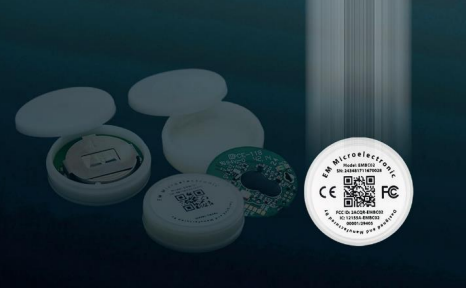
\includegraphics[width=0.7\linewidth]{ImagenesFactibilidad/beaconpic}
	\caption{Beacon EMBC22.}
	\label{fig:beacon}
\end{figure}
\Subsubsubsection{Base de Seguimiento}
Las bases de seguimiento consisten en una red de módulos receptores esparcidos por el bosque a una distancia de aproximadamente 30 metros entre sí.
Además, se hicieron las siguientes recomendaciones:
\begin{itemize}
\item Comunicación Bluetooth 5.0 para el beacon acorde al estándar, con la finalidad de poder triangular su posición.
\item Utilización de red Lora o Bluetooth 5.0 para la comunicación entre bases de seguimiento de ser necesario y con la base principal de seguimiento para reporte de datos.
\item Independencia de la red eléctrica: Utilización de paneles solares y baterías.
\end{itemize}
\begin{figure}[H]
\begin{subfigure}{.5\textwidth}
  \centering
  \includegraphics[width=.99\linewidth,page=2]{/ImagenesFactibilidad/beacon}
  \caption{Ubicación de bases de seguimiento.}
  \label{fig:sfig1}
\end{subfigure}%
\begin{subfigure}{.5\textwidth}
  \centering
  \includegraphics[width=.99\linewidth,page=3]{/ImagenesFactibilidad/beacon}
  \caption{Triangulación de posición.}
  \label{fig:sfig2}
\end{subfigure}%
\caption{Boceto de funcionamiento de las bases de seguimiento.}
\label{fig:fig}
\end{figure}
\Subsubsubsection{Base Principal de Seguimiento}
La base principal de seguimiento nuclea toda la información de las bases de seguimiento. Además, se considera la existencia de bases repetidoras para la principal en el caso de que la distancia de la red receptora sea mayor que el alcance de la base principal de seguimiento.
Esta base también debe contar con independencia de la red eléctrica y debe poder comunicarse con la base del nido mediante Bluetooth. El propósito de esta comunicación es el enviar un set de datos del ave una vez por día.
\Subsubsubsection{Propuesta de Valor Aumentada}
Cabe mencionar que al realizar el diseño sugerido, aumenta con creces la escalabilidad del producto final. Con la red de receptores desplegada, basta con utilizar un beacon en distintos animales o especies que se deseen seguir. Esto la red lo podrá hacer sin dificultad, además teniendo la capacidad de distinguir a los dispositivos de los distintos animales entre si, creando un bosque inteligente para el seguimiento de toda su fauna.
